\documentclass[a4paper]{article}

\usepackage{pdflscape}
\usepackage{multicol}
\usepackage{blindtext}
\usepackage{color}
\usepackage{enumitem}

\usepackage[left=10mm, right=10mm, top=10mm, bottom=10mm]{geometry}

\usepackage{titlesec}

\usepackage[utf8]{inputenc}
\usepackage{fourier} 
\usepackage{array}
\usepackage{makecell}

\usepackage[demo]{graphicx}



\renewcommand\theadalign{bc}
\renewcommand\theadfont{\bfseries}
\renewcommand\theadgape{\Gape[4pt]}
\renewcommand\cellgape{\Gape[4pt]}

\titlespacing\section{0pt}{5pt plus 4pt minus 2pt}{0pt plus 2pt minus 2pt}
\titlespacing\subsection{0pt}{5pt plus 4pt minus 2pt}{0pt plus 2pt minus 2pt}
\titlespacing\subsubsection{0pt}{5pt plus 4pt minus 2pt}{0pt plus 2pt minus 2pt}

\newenvironment{Figure}
  {\par\medskip\noindent\minipage{\linewidth}}
  {\endminipage\par\medskip}


\setlength{\columnseprule}{0.5pt}
\def\columnseprulecolor{\color{black}}

\pagenumbering{gobble}

\title{MuDa Cheat Sheet}
\author{Niklas Ullmann}
\date{Summer 2022}

%

\begin{document}
\begin{landscape}
    \thispagestyle{empty}

    \begin{multicols}{4}
        %
        %   Grundlagen
        %
        \section{Grundlagen}
        \begin{itemize}[noitemsep,nolistsep,leftmargin=*]
            \item Grundlagen
            \begin{itemize}[noitemsep,nolistsep,leftmargin=*]
                \item\textbf{ $Y = f(x) + \epsilon$}
                \item $Y$ = Zielgröße, $f()$ = unbekanntes/wahres Modell, $X$ = Prädiktoren, $\epsilon$ Nicht reduzierbarer Fehler
                \item \textbf{$\hat{Y} = \hat{f}(X)+\epsilon$}
                \item $\hat{Y}$ = Schätzung der Zielgröße, $\hat{f}$ = Schätzung des Modells
                \item Ziel: Möglichst genaue Schätzung finden
            \end{itemize}
            \item Ziel:
            \begin{itemize}[noitemsep,nolistsep,leftmargin=*]
                \item Prediction (Vorhersage von Werten)
                \item Inference (Ursachenanalyse, wie wirken sich Änderungen aus)
            \end{itemize}
            \item Bias-Variance Tradeoff
            \begin{itemize}[noitemsep,nolistsep,leftmargin=*]
                \item Bias: Fähigkeit des Models die eigentliche Beziehung der Daten abzubilden
                \item Variance: Fähigkeit des Models auf anderen Subsets gleich gute Modelle zu erzeugen
                \item TrainingsError: Wird immer kleiner, da Modell sich immer besser anpasst
                \item TestError: Wird erst kleiner, steigt dann aber wieder (Overfitting)
                \item Nichtreduzierbarer Error: Bleibt immer gleich (Messfehler etc.)
            \end{itemize}
        \end{itemize}
        \begin{Figure}
            \centering
            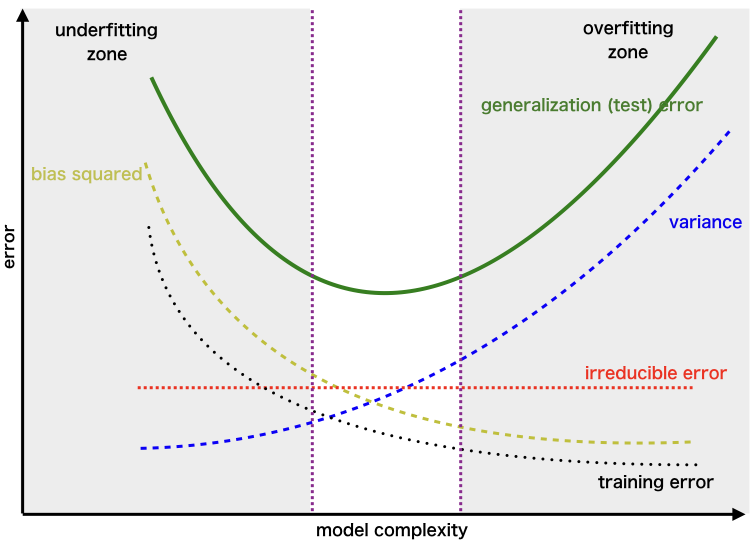
\includegraphics[width=\linewidth]{bv_tradeoff.png}
        \end{Figure}



        %
        %   Regression
        %
        \section{Regression}
        \begin{itemize}[noitemsep,nolistsep,leftmargin=*]
            \item Modellgüte:
            \begin{itemize}[noitemsep,nolistsep,leftmargin=*]
                \item Schätzung der Parameter $\beta_0 und \beta_1$ über kleinste Quadrate
                \begin{itemize}[noitemsep,nolistsep,leftmargin=*]
                    \item $\beta_1 = \frac{\sum_{i=1}^{n}(x_i-\overline{x})*(y_i-\overline{y})}{\sum_{i=1}^{n}(x_1-\overline{x})^2}$ 
                    \item $\beta_0 = \overline{y} - \beta_1\overline{x}$
                \end{itemize}
            \end{itemize}
            \item Qualitative Prädiktoren:
            \begin{itemize}[noitemsep,nolistsep,leftmargin=*]
                \item \textbf{Prädikatoren mit 2 Ausprägungen:}
                \item DummyVariable aka 0(No) oder 1 (Yes)
                \item \textcolor{red}{Achte auf Normalausprägung von R}
                \item $\hat{y} = \beta_0 + \beta_1*x_i $
                \item Koeffizient $\beta_1$ kürzt sich je nach Ausprägung raus
                \item \textbf{Prädikatoren mit $k$ Ausprägungen:}
                \item Erstelle $k-1$ Dummyvariablen
                \item Andere ist Normalzustand
            \end{itemize}
            \item Interaktionseffekte:
            \begin{itemize}[noitemsep,nolistsep,leftmargin=*]
                \item Synergieeffekte zwischen zwei oder mehreren Variablen
                \item $\hat{y}=\beta_0+\beta_1x_1+\beta_2x_2+\beta_3x_1x_2+\epsilon$
                \item Auswirkung erkennen durch Umformung:
                \item $\hat{y}=\beta_0++\beta_2x_2+ (\beta_1+\beta_3x_2)*x_1$
                \item Erhöht man $x_1$ um eine Einheit erhöht sich $\hat{y}$ um $\beta_1+\beta_3x_2$ Einheiten
                \item $x_1$ moderiert $x_2$ und Vice versa
                \item Signifikanz über p-value feststellen
                \item Interaktion zwischen Qauli udn Quanti Variablen:
                \item Kürzt sich komplett raus (wenn 0) oder ist $*1$ (wenn 1)
            \end{itemize}
        \end{itemize}


        %
        %   Klassifikation
        %
        \section{Klassifikation}
        \section{Resampling}
        \section{Modellauswahl}
        \section{R - Hilfe}
        \begin{itemize} [noitemsep,nolistsep,leftmargin=*]
            \item $set.seed(X)$ Setzt Seed für random Number Generator
            \item $c(1,2,3,4)$ Vektor mit Zahlen 1-4
            \item $df[2,3]$ Greift auf Element der 2.Reihe und 3.Spalte des DFs zu
            \item $df[,-3]$ Entfernt 3. Spalte
            \item $head()$ Zeigt erste X Zeilen von DF an
            \item $summary()$ gibt Zusammenfassung von Modellen (DF, Modelle etc.)

            \item \textbf{Modelle:}
            \begin{itemize}[noitemsep,nolistsep,leftmargin=*]
            \item $lm(A ~ B + poly(C,2) + BC)$ Lineare Regression für A mit Interaktivität von BC und C mit Exponent 2
            \item $predict(Modell, DataFrame, interval= , type= )$
                \begin{itemize}[noitemsep,nolistsep,leftmargin=*]
                    \item DF: $data.frame(x1 = c(2), x2 = c(3))$ 
                    \item $interval$ Konfidenzinterval(confidence), Prognoseinterval(prediction)
                    \item $type$ \textcolor{red}{OFFEN!}
                \end{itemize}
            \item $coef()$ Zeigt Koeffizienten des Modells
            \item $confint()$Zeigt  Konfidenzintervalle für Koeff.
            \end{itemize}

            \item \textbf{Plots:}
            \begin{itemize}[noitemsep,nolistsep,leftmargin=*]
                \item $pairs()$ Zeigt Pärchenplott aller qantitativer Variabeln
                \item $plot()$ Zeigt X/Y Plot zweier Variablen
                \item $abline(Modell, col="red")$ Zeigt Regressionslinie
                \item $qplot()$ aus ggplot2 für quickplot
            \end{itemize}
        \end{itemize}
    
    \end{multicols}
    
\end{landscape}
\end{document}